\section{zmq-broker}

A message broker prototype was developed to get a feel for how \ngrm\ 
comms services can be built as plugins communicating with messages.
This experiment builds on lessons learned from the previous PMI
investigation, implementing scalable barriers, a key-value service,
and a public interface suitable for linking with applications.

\begin{figure}
\centering
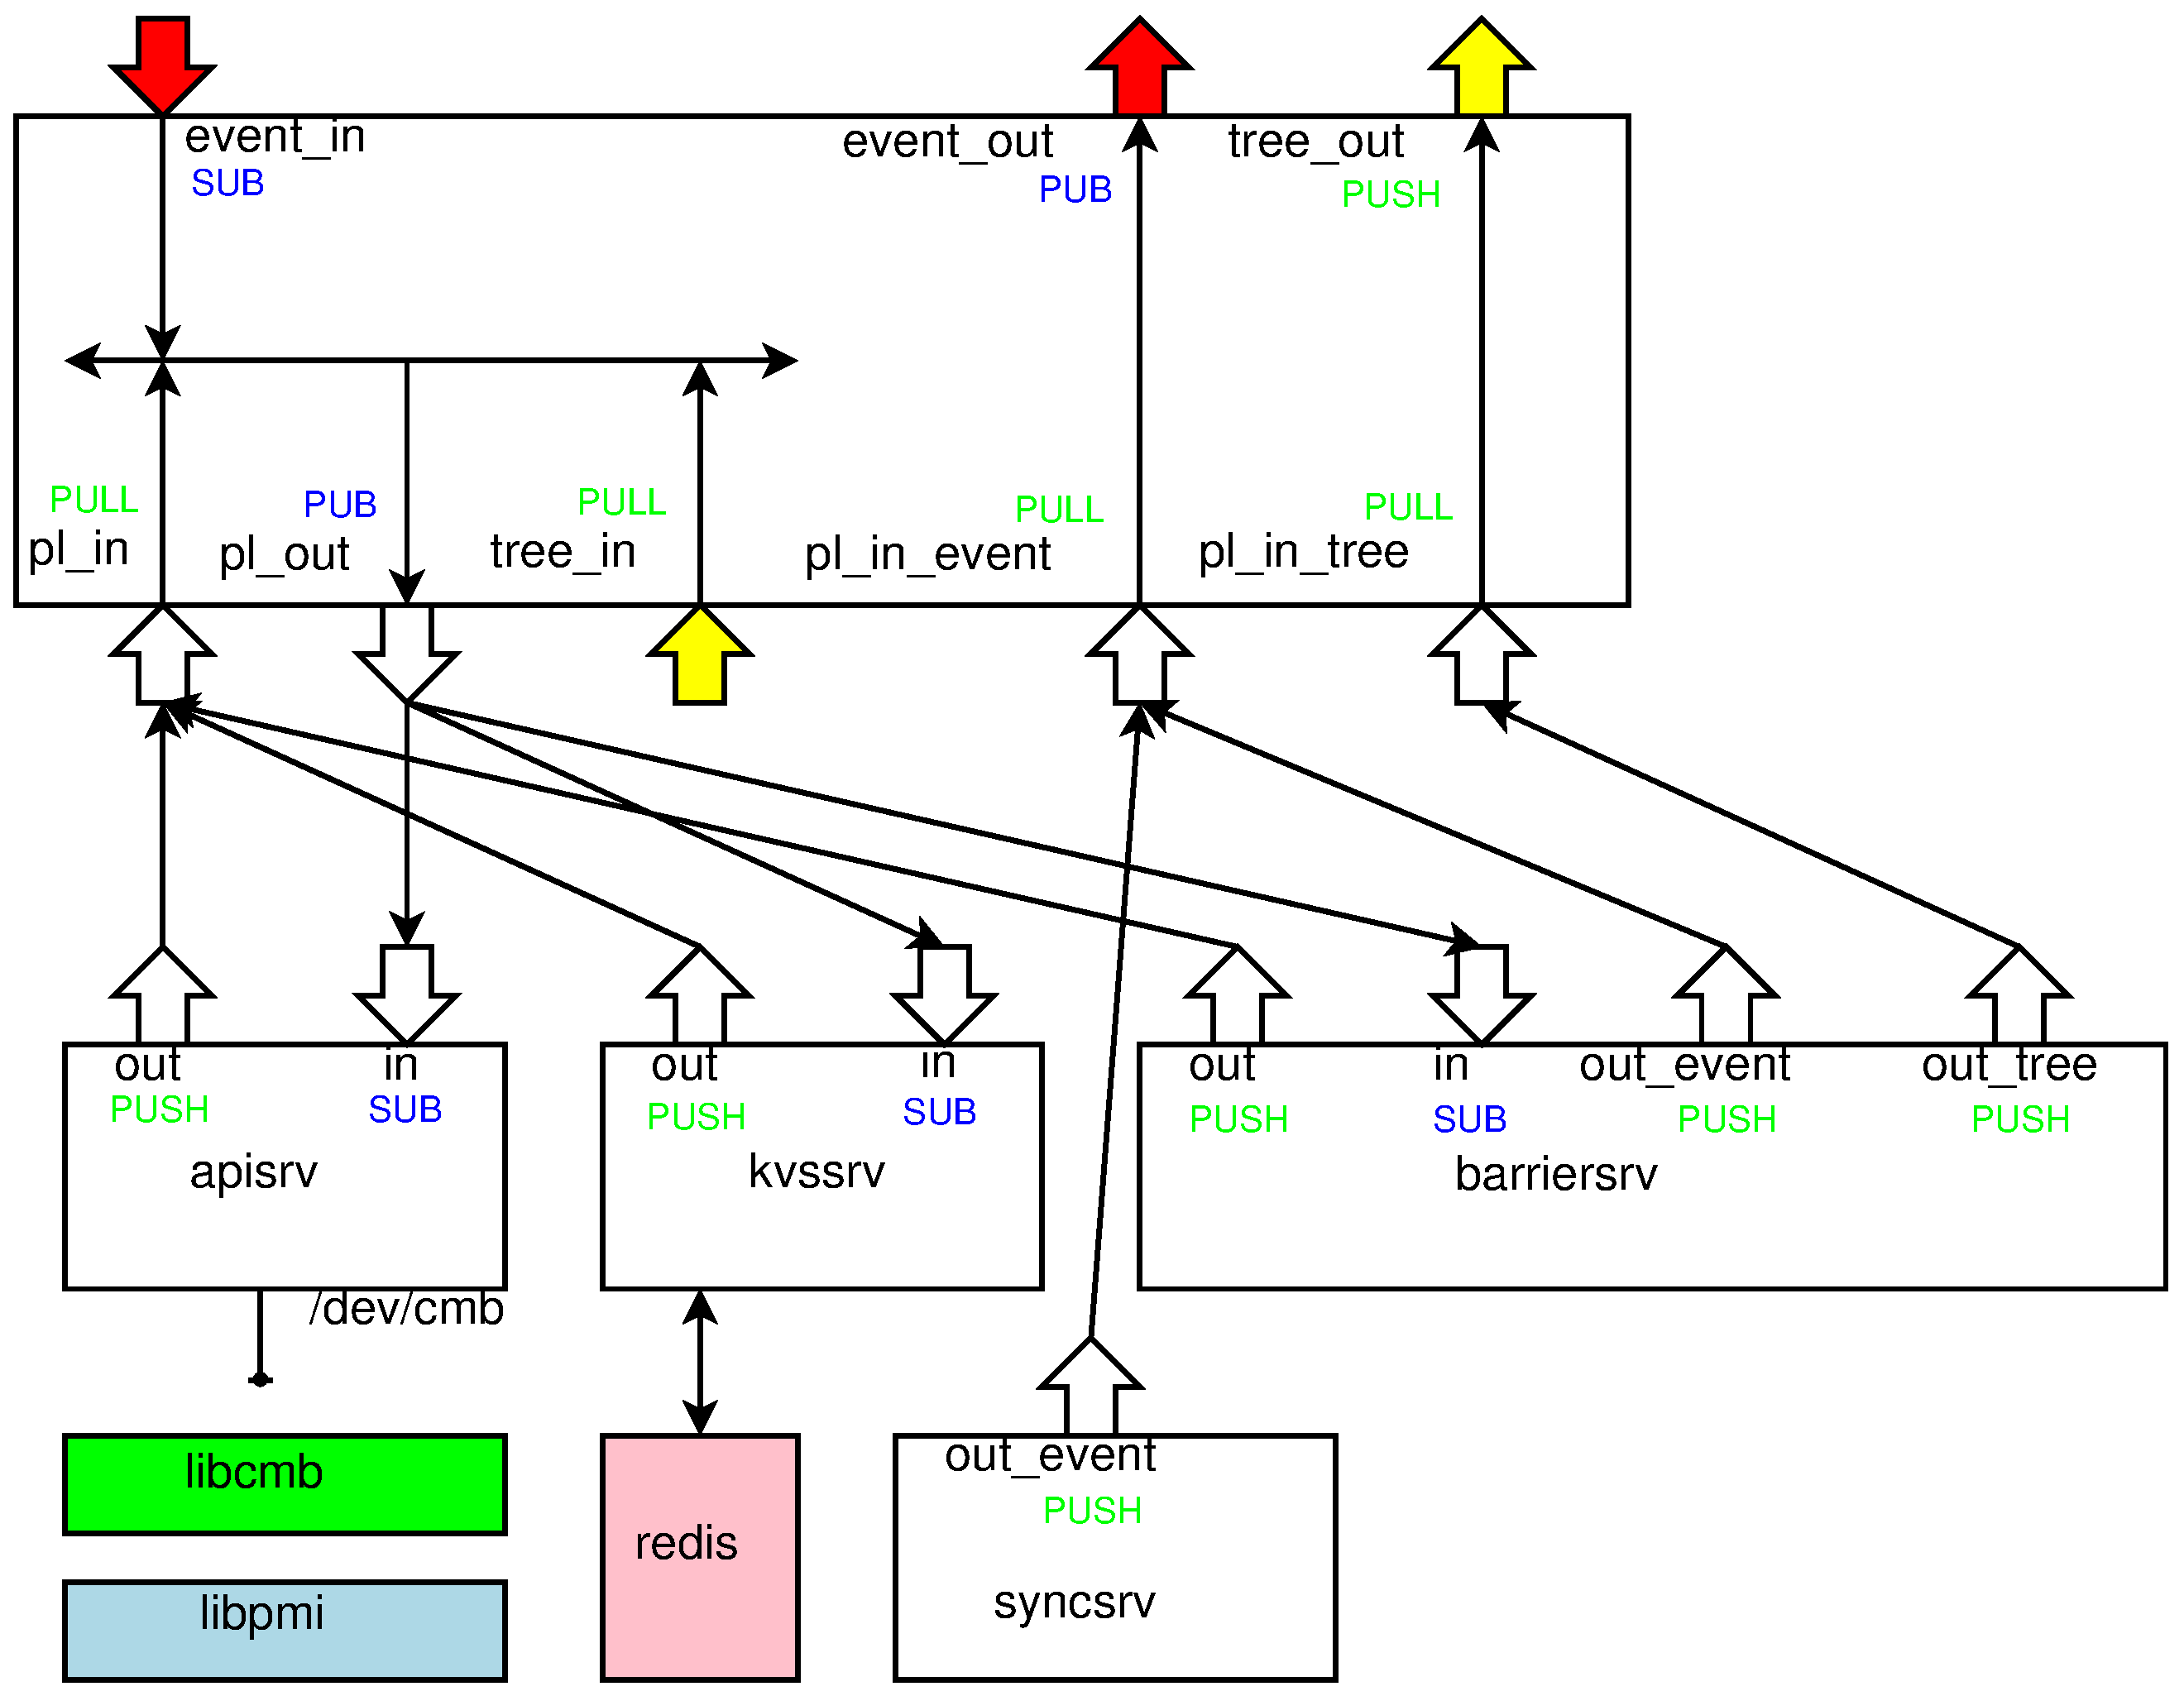
\includegraphics[scale=0.30]{zmq-broker.eps}
\caption{Broker internal architecture.  The cmbd simply routes messages
between \zMQ\ sockets, while plugins (syncsrv, apisrv, kvssrv, barriersrv)
perform specialized services.
Plugins are implemented as threads spawned by the cmbd, and communicate
with the cmbd using {\em inproc} (shared memory) \zMQ\ sockets.
The {\em libcmb} library, which provides the system's public interfaces,
communicates with the apisrv plugin via a UNIX domain socket.}
\label{fig:cmbint}
\end{figure}

\subsection{The Prototype}

The prototype consists of the cmbd message broker and plugins for various
functions.  One cmbd and a set of plugins runs on each node.
There is an internal (on-node) architecture within the process space of
the cmbd, and an external (distributed) architecture, in which the cmbds
on a collection of nodes are interconnected.  A set of communicating cmbds
roughly corresponds to a comms session as described in the \ngrm\ project
document.  Launched in concert with a \slurm\ job, the message broker
provides a scalable PMI service, and the basis to implement other services.

\subsubsection {Internal Architecture}
The internal architecture is shown in Figure~\ref{fig:cmbint}.
The cmbd acts only as a message router, passing multipart \zMQ\ messages
(Table~\ref{tab:cmbproto}) between sockets as directed by the hardwired
routes in Table~\ref{tab:cmbrouting}.
Plugins are implemented as cmbd threads that access well known \zMQ\ sockets.
Plugins generally read requests or obtain event notifications from the
{\em in} \zMQ\ socket, handle them, and write to one of the other sockets:
{\em out}, {\em out\_tree}, or {\em out\_event}.  {\em in} and {\em out}
are wired to an internal bus.  All messages routed to the bus are received
by all plugins.  {\em out\_tree} and {\em out\_event} are routed off-node.
Messages originating off-node are routed to the bus.  The following
plugins were implemented

\paragraph{apisrv}
Public interfaces, e.g. those used by PMI, are exposed by a library which
accesses the cmb through a UNIX domain socket exposed by the {\em apisrv}
plugin.   This plugin listens for connects/disconnects on the UNIX domain
socket.  When the API connects, a session is created (in the socket
{\em accept} sense), is assigned a UUID,
and a {\em event.api.uuid.connect} event is generated on the bus.
When the session disconnects by closing its socket or crashing, a
{\em event.api.uuid.disconnect} event is generated on the bus, thus
state carried by plugins for API sessions can be managed even when
sessions terminate unexpectedly.

Protocol messages are sent over the socket using a simplistic wire protocol
that enables the \zMQ\ mutipart messages used by the broker and plugins to
be encapsulated.  Some messages are interpreted by {\em apisrv} as they
arrive, for example {\em api.subscribe.tag}, {\em api.unsubscribe},
and {\em api.setuuid.uuid}.  Others are passed through to the internal
bus.  Messages arriving on the bus from other sources are sent through to
{\em apisrv} and in turn to API sessions according to the session's
subscription.  The subscription is implemented as a substring match
on the multipart message tag, identical to the way \zMQ\ implements
subscription matching on its PUB-SUB sockets.

An API sesssion messages another plugin by sending a message with a
tag accepted (subscribed to) by that plugin.
A message requiring a response includes a tag accepted by the sender
in the JSON message part.  In the API case the sender is identified as
{\em api.uuid}.  If the sender goes away between request and response,
there will be no subscriber at the sender's plugin and the response
will be discarded.

The public API functions are depicted in Table~\ref{tab:cmbapi}.

\paragraph{kvssrv}
A key-value service is implemented by the {\em kvssrv} plugin.
This plugin interfaces with the redis key-value store using the
{\em hiredis} C API.  It handles three request types: {\em kvs.get},
{\em kvs.put}, and {\em kvs.commit}.  Requests are translated into
redis transactions.  The {\em kvs.get} request is synchronous,
with the key value or error immediately returned in a reply message.
The {\em kvs.put} request is not replied to, thus an API client can
pipeline multiple {\em kvs.put} requests.
The {\em kvs.commit} request is synchronous.  Its reply includes
any errors encountered handling {\em kvs.put} transactions since the
last commit.

This plugin leverages \zMQ's built-in message queues.  The plugin thread
simply loops, reading one request, handling the associated redis trasaction,
and sending a reply, if any.  Pipelined requests accumulate in the \zMQ\ 
{\em in} socket queue and are handled in the order received, thus a
{\em kvs.commit} enqueued behind a set of {\em kvs.put} requests need
not do anything complicated to ensure the {\em kvs.put}'s have completed 
when it is finally handled by the {\em kvssrv} thread.

In order to track {\em kvs.put} errors for each API session so that a
{\em kvs.commit} can return them, {\em kvssrv} must maintain state per
API session.  When this state is created, {\em kvssrv} subscribes to
the session's {\em api.uuid.disconnect} message so that it can free
the state when the session terminates.

In order to implement the PMI shared key-value space {\em kvssrv}
is set up to connect to a single instance of redis for the job.
Since there will be one redis connection per node, scalability is improved
over the {\em pmi-redis} prototype which had two redis connections per
MPI task.  However, scalability will still be limited by the number
of simultaneous hiredis connections that a single redis server can handle.

\paragraph{barriersrv}
The {\em barriersrv} plugin implements barriers using the reduction
tree described below.   The {\tt cmb\_barrier()} API function requires
all participants to provide identical {\em name} and {\em nprocs} arguments.
This is translated into a {\em barrier.enter.name} message to the local
{\em barriersrv} plugin, which creates a local context for the barrier
if one does not already exist.  The API then blocks waiting for a
{\em event.barrier.exit.name} message.

Each message received for the barrier by {\em barriersrv} increments
an internal count in the context.  If the count reaches nprocs,
a {\em event.barrier.exit.name} message is generated.  This is published
session-wide and causes all the API barrier calls for the named barrier
to return.  Alternatively, if nprocs is not reached before a 2ms timer
expires, {\em barriersrv} pushes a {\em barrier.enter.name} message upstream
containing the current count, which it then clears.  Eventually, the upstream
count reaches nprocs and the barrier is terminated.  Upon receipt of the
exit message, {\em barriersrv} removes its context for the barrier.

TODO: implement {\em event.barrier.fail.name} in case a call is made with
the wrong nprocs value, or a local API client exits before the barrier is
complete.

\paragraph{syncsrv}
This plugin is only run on the node at the root of the reduction tree.
It generates a periodic multicast message, {\em event.sched.trigger},
that is received job wide.  The API call {\tt cmb\_sync} simply blocks waiting
for the next occurrence of this message.  This provides a mechanism to execute
"overhead" tasks simultaneously across the job to minimize their impact on
noise sensitive MPI jobs.

\begin{table}
\centering
\begin{tabular}{|l|l|l|l|}\hline
\textbf{Plugin-sock} & \textbf{CMB-sock} & \textbf{CMB-sock}
					 & \textbf{External} \\
\hline
out (PUSH)		& pl\_in (PULL)	& {\em BUS} & \\
out\_event (PUSH)  & pl\_in\_event (PULL) & event\_out (PUB) & $\rightarrow$ \\
out\_tree (PUSH) & pl\_in\_tree	(PULL) & tree\_out (PUSH) & $\rightarrow$ \\
in (SUB)	& pl\_out (PUB)	& {\em BUS}     & \\
\hline
		& {\em BUS}	& event\_in (SUB) & $\leftarrow$ \\
		& {\em BUS}	& tree\_in (PULL) & $\leftarrow$ \\
\hline
\end{tabular}
\caption{The cmbd internal routing table.}
\label{tab:cmbrouting}
\end{table}

\begin{table}
\centering
\begin{tabular}{|l|p{6cm}|}\hline
\textbf{message part} & \textbf{example} \\
\hline
{\em tag} & {\tt barrier.enter.job22-1} \\
\hline
{\em json} & {\tt \{ "count" : 1, "nprocs" : 16 \} }\\
\hline
{\em data} & nil\\
\hline
\end{tabular}
\caption{Message protocol.  Messages consist of three \zMQ\ message parts.
The first part is a {\em tag} formatted as a \zMQ\ string suitable for
use as a subscription tag on PUB-SUB sockets, and which is used to identify
the recipient(s).
The second part (optional) is JSON formatted as a \zMQ\ string.
The third part (optional) is raw data, needed since JSON has no opaque
data type.}
\label{tab:cmbproto}
\end{table}

\subsubsection {External Architecture}
The cmbd implements the reduction network and event service described
in the \ngrm\ comms design.

\begin{figure}
\centering
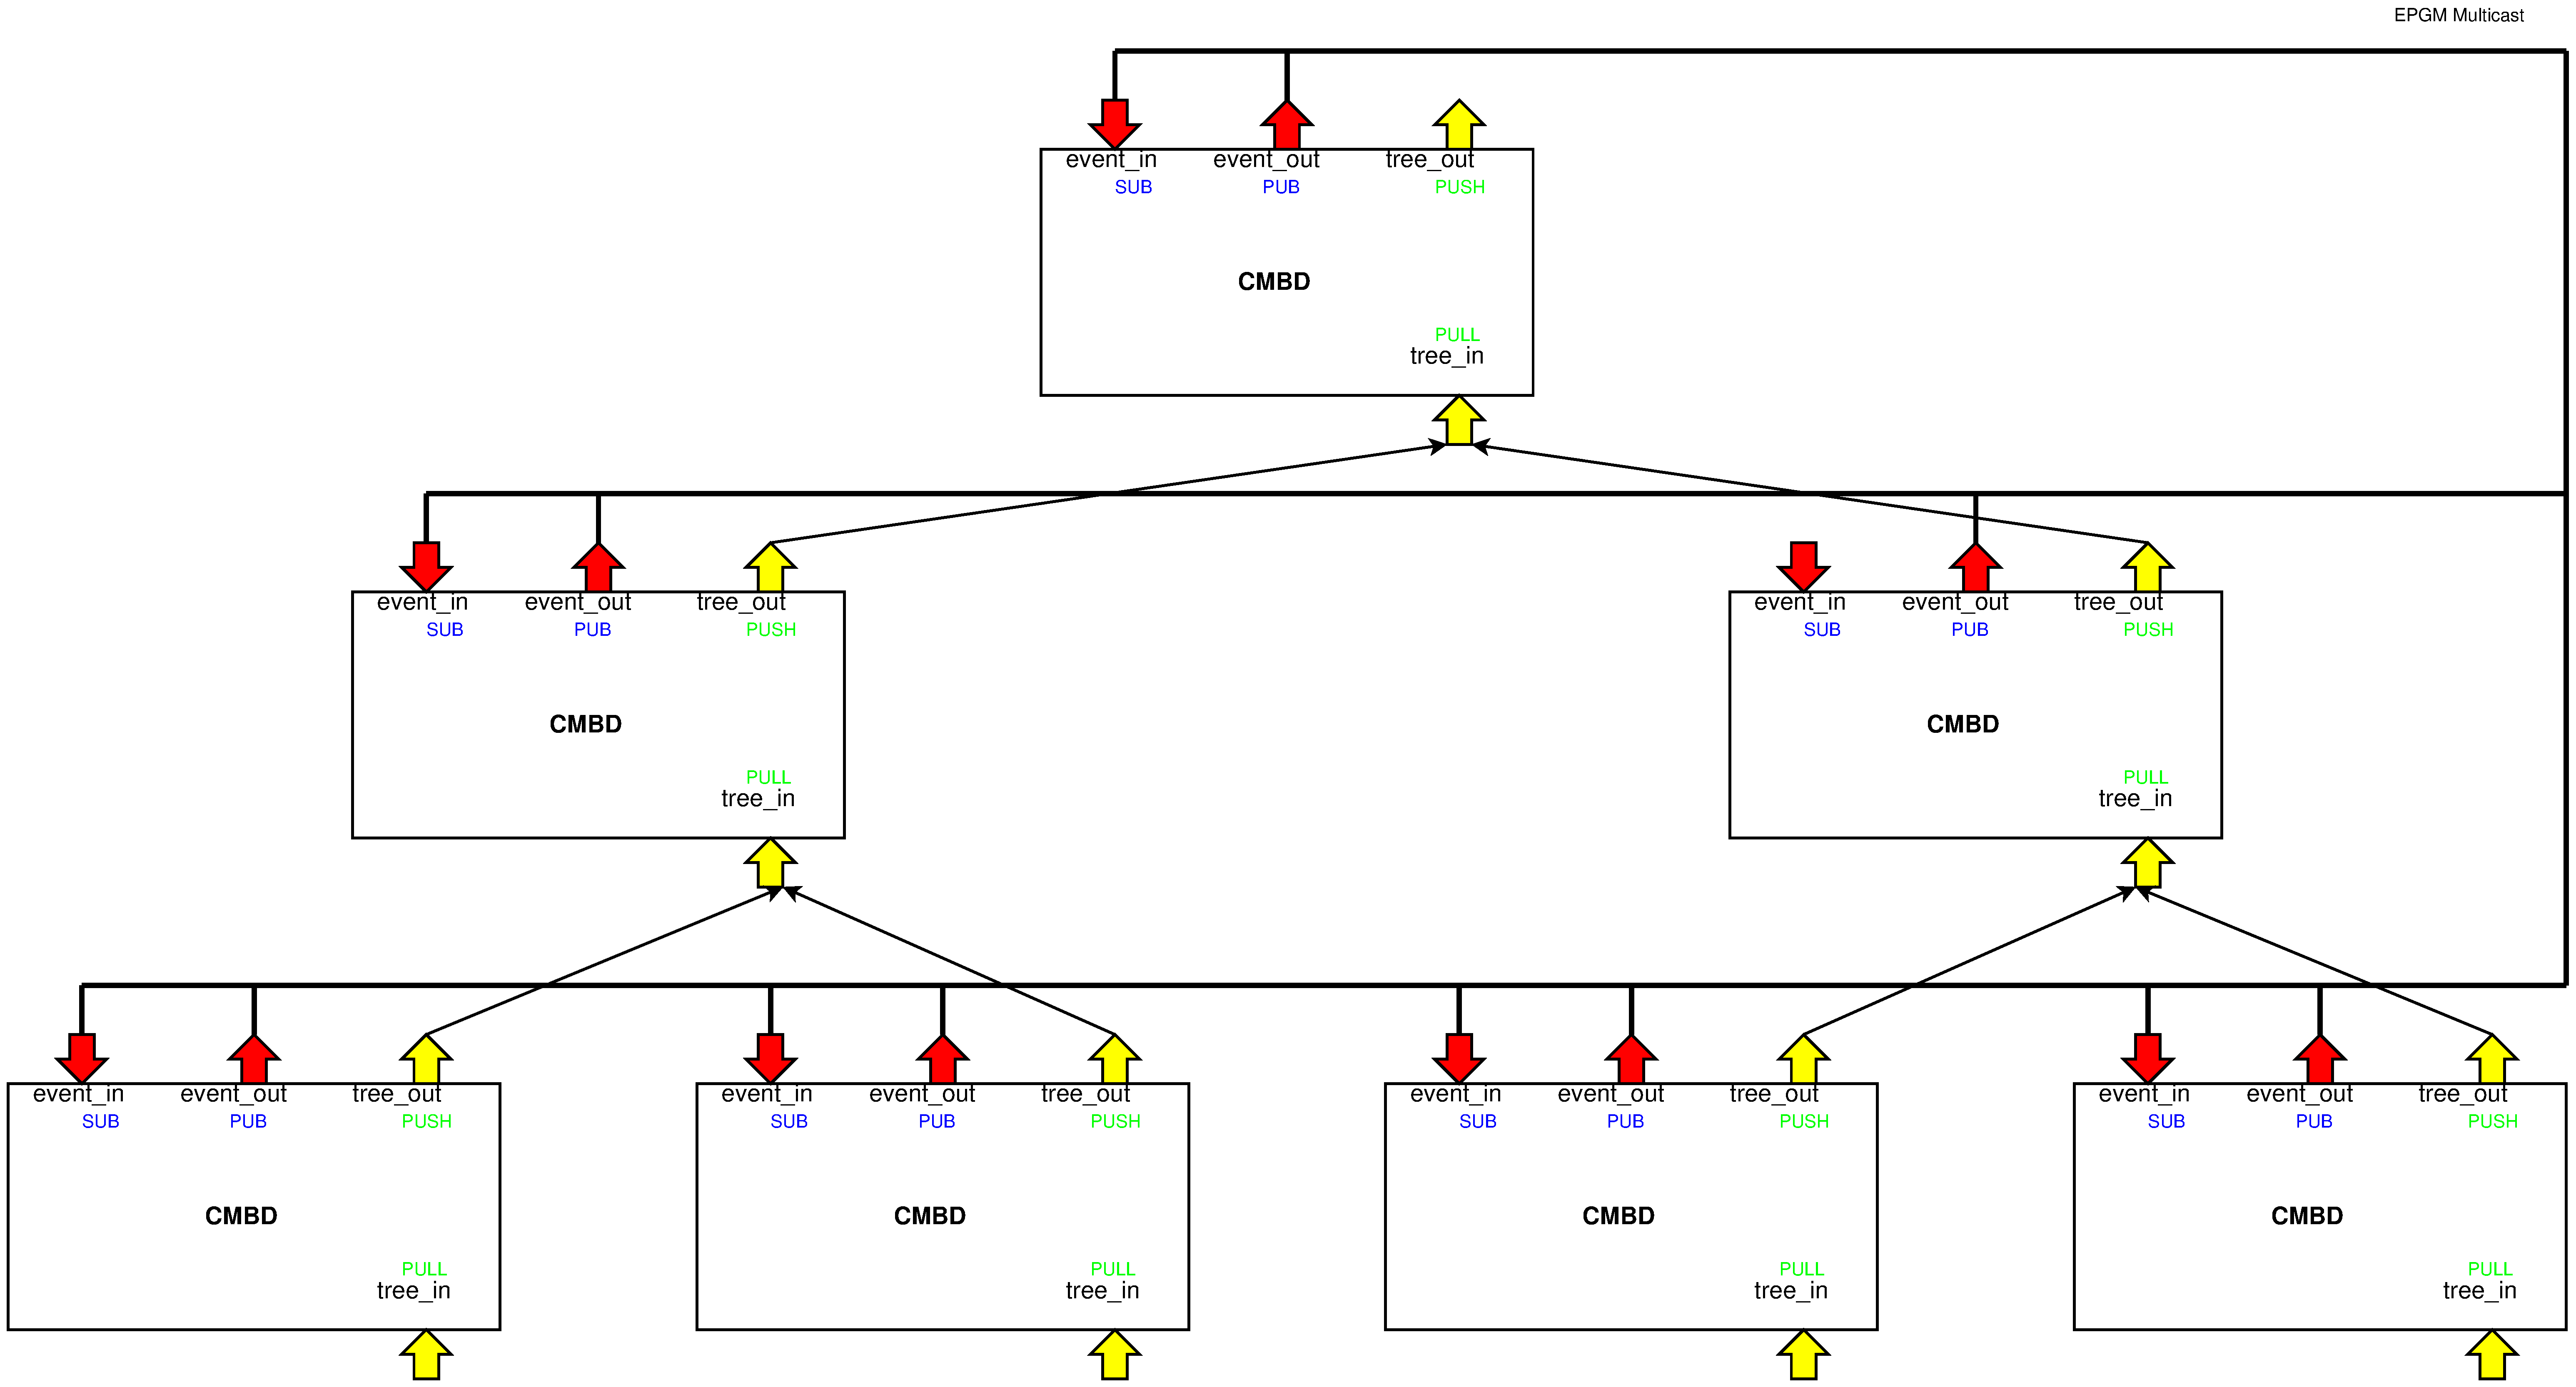
\includegraphics[scale=0.15]{zmq-broker-tree.eps}
\caption{Broker external architecture.}
\label{fig:cmbext}
\end{figure}


\begin{table}
\centering
\begin{tabular}{|p{0.7cm}p{5cm}|p{9cm}|}\hline
\multicolumn{2}{|l|}{\textbf{Function}}
  & \textbf{Description} \\
\hline
{\tt cmb\_t} & {\tt cmb\_init (void)}
  & Create a {\em cmb\_t} context for communicating with the broker.\\
{\tt void} & {\tt cmb\_fini (cmb\_t c)}
  & Destroy a {\em cmb\_t} context.\\
\hline
{\tt int} & {\tt cmb\_ping (cmb\_t c, int seq, int padding)}
  & Send a ping message to the broker's internal bus and wait for it
    to be echoed back.  {\em padding} bytes of payload will be added to
    the message.
    On success, returns $0$; on failure, returns $-1$ with errno set.\\
\hline
{\tt int} & {\tt cmb\_snoop (cmb\_t c, char {*sub})}
  & Print all messages on the broker's internal bus whose tags match the
    subscription string {\em sub}.  The empty string matches all messages.
    On success, does not return; on failure, returns $-1$ with errno set.\\
\hline
{\tt int}
  & {\tt cmb\_barrier (cmb\_t c, char {*name}, int nprocs)}
  & Execute barrier {\em name}.  The call blocks until {\em nprocs}
    processes have entered the barrier.  
    All processes entering a given barrier must call this function with
    identical arguments.
    On success, returns $0$; on failure, returns $-1$ with errno set.\\
\hline
{\tt int}
  & {\tt cmb\_sync (cmb\_t c)}
  & Block until {\em event.sched.trigger} is received.  This event is
    a job-wide, periodic multicast signal used to synchronize system noise.
    By default it is sent out every $10s$.
    On success, returns $0$; on failure, returns $-1$ with errno set.\\
\hline
{\tt int}
  & {\tt cmb\_kvs\_put (cmb\_t c, char {*key}, char {*val})}
  & Set {\em key} to {\em val} in the job-wide key-value store.
    If the key already has a value, it is overwritten.
    Errors resulting from the actual KVS transaction are not reported
    until the next {\em cmb\_kvs\_commit} call.
    On success, returns $0$; on failure, returns $-1$ with errno set.\\
{\tt {char*}}
  & {\tt cmb\_kvs\_get (cmb\_t c, char {*key})}
  & Retrieve the value of {\em key} from the job-wide key-value store.
    On success, returns a copy of value which the caller must free;
    on failure, returns NULL with errno set.\\
{\tt int}
  & {\tt cmb\_kvs\_commit (cmb\_t c, int *errcount, int *putcount)}
  & Block until the job-wide key-value store has completed all transactions
    originating on the local node.  {\em putcount} will contain the number
    of {\em cmb\_kvs\_put} calls executed by this context since the last commit.
    {\em errcount} will contian the number of failed puts since the last commit.
    On success, returns $0$; on failure, returns $-1$ with errno set.\\
\hline
\end{tabular}
\caption{Public interfaces exported by the broker.  Users would
{\tt \#include "cmb.h"} and link {\tt -lcmb}.  {\em libcmb} utilizes
a UNIX domain socket exported by the {\em apisrv} plugin to implement
a very lightweight interface suitable for linking with applications such
as MPI runtimes (\zMQ\ is too heavyweight to be used directly by applications.)}
\label{tab:cmbapi}
\end{table}

\subsection{Conclusions}

\paragraph{\zMQ\ pub-sub limitations} \zMQ\ pub-sub sockets drop messages when
their internal queues reach a high water mark.\footnote{The {\tt ZMQ\_SNDHWM}
defaults to 1000 messages in \zMQ\ 3.2 but can be changed via
{\tt zmq\_setsockopt()}, called before {\tt zmq\_bind()} or
{\tt zmq\_connect()}}.
They cannot be configured to block the sender.  This makes pub-sub
the inappropriate socket type for {\em pl\_out} in the prototype as
important messages (e.g. kvs put or commit) can be dropped if the
plumbing backs up.
It is likely appropriate for event distribution but one must be careful
to limit the volume of events loosed in the system.

\paragraph{\zMQ\ PGM transport}  The PGM/EPGM transport is rate limited by
default to $100 Kbytes/sec$, although this is tunable by a socket option.
Some versions of \zMQ\ seem to have better OpenPGM integration than others.
Although PGM is reliable, pub-sub can lose messages as described above.

\paragraph{Flow control}  The prototype implements no flow control.
The broker's single thread can block if the internal queues for push-pull
sockets fill up, since we only make blocking {\tt zmq\_msg\_send} calls.
Some sort of flow control in combination with non-blocking sends needs to
be implemented.

\paragraph{JSON limitations}  JSON has no reasonable way to represent
a byte array.  In general JSON is not compact, but byte arrays are truly
ridiculous as a way of representing opaque data.  One could use base64
encoding within JSON strings.  We used an opaque \zMQ\ message part.
